\begin{figure}
\centering
  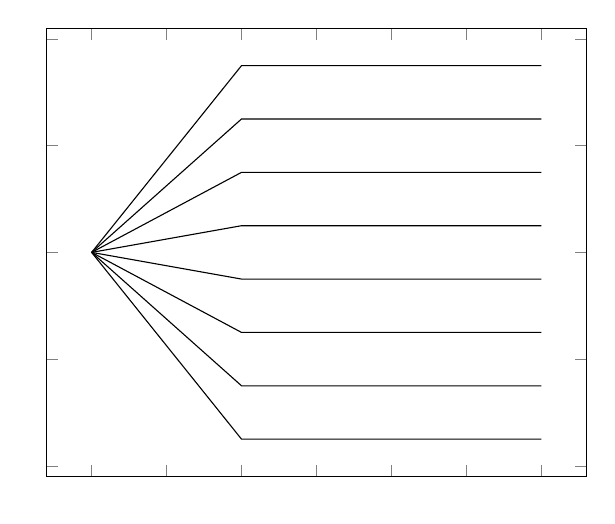
\begin{tikzpicture}
    \begin{axis}[xticklabels={,,},yticklabels={,,}]
      \addplot [color=black] coordinates {
        (1, 0)
        (2, -3.5)
        (3, -3.5)
        (4, -3.5)
      };
      \addplot [color=black] coordinates {
        (1, 0)
        (2, -2.5)
        (3, -2.5)
        (4, -2.5)
      };
      \addplot [color=black] coordinates {
        (1, 0)
        (2, -1.5)
        (3, -1.5)
        (4, -1.5)
      };
      \addplot [color=black] coordinates {
        (1, 0)
        (2, -0.5)
        (3, -0.5)
        (4, -0.5)
      };
      \addplot [color=black] coordinates {
        (1, 0)
        (2, 0.5)
        (3, 0.5)
        (4, 0.5)
      };
      \addplot [color=black] coordinates {
        (1, 0)
        (2, 1.5)
        (3, 1.5)
        (4, 1.5)
      };
      \addplot [color=black] coordinates {
        (1, 0)
        (2, 2.5)
        (3, 2.5)
        (4, 2.5)
      };
      \addplot [color=black] coordinates {
        (1, 0)
        (2, 3.5)
        (3, 3.5)
        (4, 3.5)
      };
    \end{axis}
  \end{tikzpicture}
  % begin of figure 2
  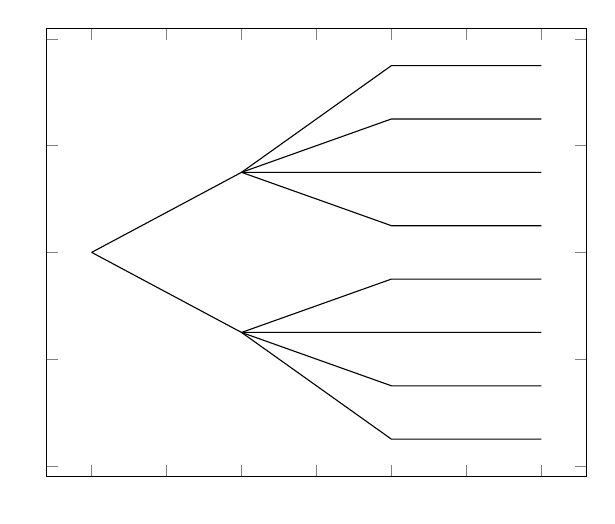
\begin{tikzpicture}
    \begin{axis}[xticklabels={,,},yticklabels={,,}]
      \addplot [color=black] coordinates {
        (2, -1.5)
        (3, -3.5)
        (4, -3.5)
      };
      \addplot [color=black] coordinates {
        (2, -1.5)
        (3, -2.5)
        (4, -2.5)
      };
      \addplot [color=black] coordinates {
        (1, 0)
        (2, -1.5)
        (3, -1.5)
        (4, -1.5)
      };
      \addplot [color=black] coordinates {
        (2, -1.5)
        (3, -0.5)
        (4, -0.5)
      };
      \addplot [color=black] coordinates {
        (2, 1.5)
        (3, 0.5)
        (4, 0.5)
      };
      \addplot [color=black] coordinates {
        (1, 0)
        (2, 1.5)
        (3, 1.5)
        (4, 1.5)
      };
      \addplot [color=black] coordinates {
        (2, 1.5)
        (3, 2.5)
        (4, 2.5)
      };
      \addplot [color=black] coordinates {
        (2, 1.5)
        (3, 3.5)
        (4, 3.5)
      };
    \end{axis}
  \end{tikzpicture}
  % begin of figure 3
  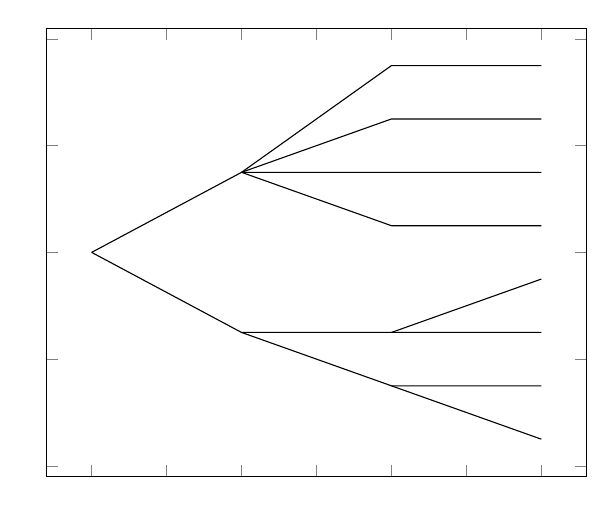
\begin{tikzpicture}
    \begin{axis}[xticklabels={,,},yticklabels={,,}]
      \addplot [color=black] coordinates {
        (3, -2.5)
        (4, -3.5)
      };
      \addplot [color=black] coordinates {
        (2, -1.5)
        (3, -2.5)
        (4, -2.5)
      };
      \addplot [color=black] coordinates {
        (1, 0)
        (2, -1.5)
        (3, -1.5)
        (4, -1.5)
      };
      \addplot [color=black] coordinates {
        (3, -1.5)
        (4, -0.5)
      };
      \addplot [color=black] coordinates {
        (2, 1.5)
        (3, 0.5)
        (4, 0.5)
      };
      \addplot [color=black] coordinates {
        (1, 0)
        (2, 1.5)
        (3, 1.5)
        (4, 1.5)
      };
      \addplot [color=black] coordinates {
        (2, 1.5)
        (3, 2.5)
        (4, 2.5)
      };
      \addplot [color=black] coordinates {
        (2, 1.5)
        (3, 3.5)
        (4, 3.5)
      };
    \end{axis}
  \end{tikzpicture}
  % begin of figure 4
  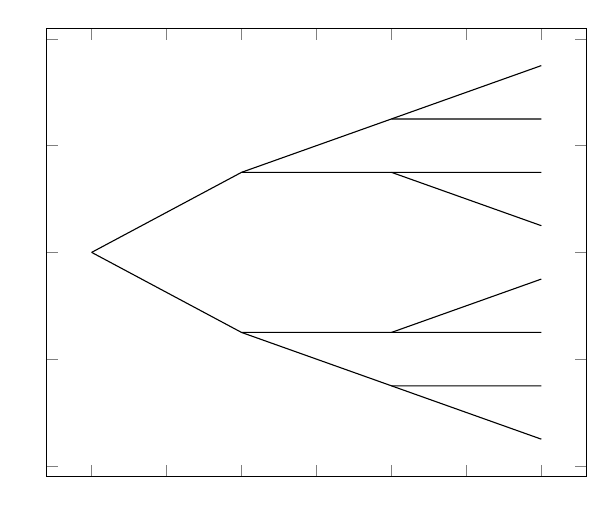
\begin{tikzpicture}
    \begin{axis}[xticklabels={,,},yticklabels={,,}]
      \addplot [color=black] coordinates {
        (3, -2.5)
        (4, -3.5)
      };
      \addplot [color=black] coordinates {
        (2, -1.5)
        (3, -2.5)
        (4, -2.5)
      };
      \addplot [color=black] coordinates {
        (1, 0)
        (2, -1.5)
        (3, -1.5)
        (4, -1.5)
      };
      \addplot [color=black] coordinates {
        (3, -1.5)
        (4, -0.5)
      };
      \addplot [color=black] coordinates {
        (3, 1.5)
        (4, 0.5)
      };
      \addplot [color=black] coordinates {
        (1, 0)
        (2, 1.5)
        (3, 1.5)
        (4, 1.5)
      };
      \addplot [color=black] coordinates {
        (2, 1.5)
        (3, 2.5)
        (4, 2.5)
      };
      \addplot [color=black] coordinates {
        (3, 2.5)
        (4, 3.5)
      };
    \end{axis}
  \end{tikzpicture}
  \caption{Evolution of the stage-wise MILP algorithm for a tree with two branches to each node.
    Top left: The tree is initialized with only the root node.
    Top right: After solving the MILP of the root node.
    Bottom left: After solving the lower of the two second stage nodes.
    Bottom right: The tree, completely solved.
  }
  \label{fig:swmilp-explanation}
\end{figure}
%%% Local Variables:
%%% mode: latex
%%% TeX-master: "da"
%%% End:
